\documentclass[12pt]{article}
%Fall 2022
% Some basic packages
\usepackage{standalone}[subpreambles=true]
\usepackage[utf8]{inputenc}
\usepackage[T1]{fontenc}
\usepackage{textcomp}
\usepackage[english]{babel}
\usepackage{url}
\usepackage{graphicx}
%\usepackage{quiver}
\usepackage{float}
\usepackage{enumitem}
\usepackage{lmodern}
\usepackage{comment}
\usepackage{hyperref}
\usepackage[usenames,svgnames,dvipsnames]{xcolor}
\usepackage[margin=1in]{geometry}
\usepackage{pdfpages}

\pdfminorversion=7

% Don't indent paragraphs, leave some space between them
\usepackage{parskip}

% Hide page number when page is empty
\usepackage{emptypage}
\usepackage{subcaption}
\usepackage{multicol}
\usepackage[b]{esvect}

% Math stuff
\usepackage{amsmath, amsfonts, mathtools, amsthm, amssymb}
\usepackage{bbm}
\usepackage{stmaryrd}
\allowdisplaybreaks

% Fancy script capitals
\usepackage{mathrsfs}
\usepackage{cancel}
% Bold math
\usepackage{bm}
% Some shortcuts
\newcommand{\rr}{\ensuremath{\mathbb{R}}}
\newcommand{\zz}{\ensuremath{\mathbb{Z}}}
\newcommand{\qq}{\ensuremath{\mathbb{Q}}}
\newcommand{\nn}{\ensuremath{\mathbb{N}}}
\newcommand{\ff}{\ensuremath{\mathbb{F}}}
\newcommand{\cc}{\ensuremath{\mathbb{C}}}
\newcommand{\ee}{\ensuremath{\mathbb{E}}}
\newcommand{\hh}{\ensuremath{\mathbb{H}}}
\renewcommand\O{\ensuremath{\emptyset}}
\newcommand{\norm}[1]{{\left\lVert{#1}\right\rVert}}
\newcommand{\dbracket}[1]{{\left\llbracket{#1}\right\rrbracket}}
\newcommand{\ve}[1]{{\bm{#1}}}
\newcommand\allbold[1]{{\boldmath\textbf{#1}}}
\DeclareMathOperator{\lcm}{lcm}
\DeclareMathOperator{\im}{im}
\DeclareMathOperator{\coim}{coim}
\DeclareMathOperator{\dom}{dom}
\DeclareMathOperator{\tr}{tr}
\DeclareMathOperator{\rank}{rank}
\DeclareMathOperator*{\var}{Var}
\DeclareMathOperator*{\ev}{E}
\DeclareMathOperator{\dg}{deg}
\DeclareMathOperator{\aff}{aff}
\DeclareMathOperator{\conv}{conv}
\DeclareMathOperator{\inte}{int}
\DeclareMathOperator*{\argmin}{argmin}
\DeclareMathOperator*{\argmax}{argmax}
\DeclareMathOperator{\graph}{graph}
\DeclareMathOperator{\sgn}{sgn}
\DeclareMathOperator*{\Rep}{Rep}
\DeclareMathOperator{\Proj}{Proj}
\DeclareMathOperator{\mat}{mat}
\DeclareMathOperator{\diag}{diag}
\DeclareMathOperator{\aut}{Aut}
\DeclareMathOperator{\gal}{Gal}
\DeclareMathOperator{\inn}{Inn}
\DeclareMathOperator{\edm}{End}
\DeclareMathOperator{\Hom}{Hom}
\DeclareMathOperator{\ext}{Ext}
\DeclareMathOperator{\tor}{Tor}
\DeclareMathOperator{\Span}{Span}
\DeclareMathOperator{\Stab}{Stab}
\DeclareMathOperator{\cont}{cont}
\DeclareMathOperator{\Ann}{Ann}
\DeclareMathOperator{\Div}{div}
\DeclareMathOperator{\curl}{curl}
\DeclareMathOperator{\nat}{Nat}
\DeclareMathOperator{\gr}{Gr}
\DeclareMathOperator{\vect}{Vect}
\DeclareMathOperator{\id}{id}
\DeclareMathOperator{\Mod}{Mod}
\DeclareMathOperator{\sign}{sign}
\DeclareMathOperator{\Surf}{Surf}
\DeclareMathOperator{\fcone}{fcone}
\DeclareMathOperator{\Rot}{Rot}
\DeclareMathOperator{\grad}{grad}
\DeclareMathOperator{\atan2}{atan2}
\DeclareMathOperator{\Ric}{Ric}
\let\vec\relax
\DeclareMathOperator{\vec}{vec}
\let\Re\relax
\DeclareMathOperator{\Re}{Re}
\let\Im\relax
\DeclareMathOperator{\Im}{Im}
% Put x \to \infty below \lim
\let\svlim\lim\def\lim{\svlim\limits}

%wide hat
\usepackage{scalerel,stackengine}
\stackMath
\newcommand*\wh[1]{%
\savestack{\tmpbox}{\stretchto{%
  \scaleto{%
    \scalerel*[\widthof{\ensuremath{#1}}]{\kern-.6pt\bigwedge\kern-.6pt}%
    {\rule[-\textheight/2]{1ex}{\textheight}}%WIDTH-LIMITED BIG WEDGE
  }{\textheight}% 
}{0.5ex}}%
\stackon[1pt]{#1}{\tmpbox}%
}
\parskip 1ex

%Make implies and impliedby shorter
\let\implies\Rightarrow
\let\impliedby\Leftarrow
\let\iff\Leftrightarrow
\let\epsilon\varepsilon

% Add \contra symbol to denote contradiction
\usepackage{stmaryrd} % for \lightning
\newcommand\contra{\scalebox{1.5}{$\lightning$}}

% \let\phi\varphi

% Command for short corrections
% Usage: 1+1=\correct{3}{2}

\definecolor{correct}{HTML}{009900}
\newcommand\correct[2]{\ensuremath{\:}{\color{red}{#1}}\ensuremath{\to }{\color{correct}{#2}}\ensuremath{\:}}
\newcommand\green[1]{{\color{correct}{#1}}}

% horizontal rule
\newcommand\hr{
    \noindent\rule[0.5ex]{\linewidth}{0.5pt}
}

% hide parts
\newcommand\hide[1]{}

% si unitx
\usepackage{siunitx}
\sisetup{locale = FR}

%allows pmatrix to stretch
\makeatletter
\renewcommand*\env@matrix[1][\arraystretch]{%
  \edef\arraystretch{#1}%
  \hskip -\arraycolsep
  \let\@ifnextchar\new@ifnextchar
  \array{*\c@MaxMatrixCols c}}
\makeatother

\renewcommand{\arraystretch}{0.8}

\renewcommand{\baselinestretch}{1.5}

\usepackage{graphics}
\usepackage{epstopdf}

\RequirePackage{hyperref}
%%
%% Add support for color in order to color the hyperlinks.
%% 
\hypersetup{
  colorlinks = true,
  urlcolor = blue,
  citecolor = blue
}
%%fakesection Links
\hypersetup{
    colorlinks,
    linkcolor={red!50!black},
    citecolor={green!50!black},
    urlcolor={blue!80!black}
}
%customization of cleveref
\RequirePackage[capitalize,nameinlink]{cleveref}[0.19]

% Per SIAM Style Manual, "section" should be lowercase
\crefname{section}{section}{sections}
\crefname{subsection}{subsection}{subsections}
\Crefname{section}{Section}{Sections}
\Crefname{subsection}{Subsection}{Subsections}

% Per SIAM Style Manual, "Figure" should be spelled out in references
\Crefname{figure}{Figure}{Figures}

% Per SIAM Style Manual, don't say equation in front on an equation.
\crefformat{equation}{\textup{#2(#1)#3}}
\crefrangeformat{equation}{\textup{#3(#1)#4--#5(#2)#6}}
\crefmultiformat{equation}{\textup{#2(#1)#3}}{ and \textup{#2(#1)#3}}
{, \textup{#2(#1)#3}}{, and \textup{#2(#1)#3}}
\crefrangemultiformat{equation}{\textup{#3(#1)#4--#5(#2)#6}}%
{ and \textup{#3(#1)#4--#5(#2)#6}}{, \textup{#3(#1)#4--#5(#2)#6}}{, and \textup{#3(#1)#4--#5(#2)#6}}

% But spell it out at the beginning of a sentence.
\Crefformat{equation}{#2Equation~\textup{(#1)}#3}
\Crefrangeformat{equation}{Equations~\textup{#3(#1)#4--#5(#2)#6}}
\Crefmultiformat{equation}{Equations~\textup{#2(#1)#3}}{ and \textup{#2(#1)#3}}
{, \textup{#2(#1)#3}}{, and \textup{#2(#1)#3}}
\Crefrangemultiformat{equation}{Equations~\textup{#3(#1)#4--#5(#2)#6}}%
{ and \textup{#3(#1)#4--#5(#2)#6}}{, \textup{#3(#1)#4--#5(#2)#6}}{, and \textup{#3(#1)#4--#5(#2)#6}}

% Make number non-italic in any environment.
\crefdefaultlabelformat{#2\textup{#1}#3}

% Environments
\makeatother
% For box around Definition, Theorem, \ldots
%%fakesection Theorems
\usepackage{thmtools}
\usepackage[framemethod=TikZ]{mdframed}

\theoremstyle{definition}
\mdfdefinestyle{mdbluebox}{%
	roundcorner = 10pt,
	linewidth=1pt,
	skipabove=12pt,
	innerbottommargin=9pt,
	skipbelow=2pt,
	nobreak=true,
	linecolor=blue,
	backgroundcolor=TealBlue!5,
}
\declaretheoremstyle[
	headfont=\sffamily\bfseries\color{MidnightBlue},
	mdframed={style=mdbluebox},
	headpunct={\\[3pt]},
	postheadspace={0pt}
]{thmbluebox}

\mdfdefinestyle{mdredbox}{%
	linewidth=0.5pt,
	skipabove=12pt,
	frametitleaboveskip=5pt,
	frametitlebelowskip=0pt,
	skipbelow=2pt,
	frametitlefont=\bfseries,
	innertopmargin=4pt,
	innerbottommargin=8pt,
	nobreak=false,
	linecolor=RawSienna,
	backgroundcolor=Salmon!5,
}
\declaretheoremstyle[
	headfont=\bfseries\color{RawSienna},
	mdframed={style=mdredbox},
	headpunct={\\[3pt]},
	postheadspace={0pt},
]{thmredbox}

\declaretheorem[%
style=thmbluebox,name=Theorem,numberwithin=section]{thm}
\declaretheorem[style=thmbluebox,name=Lemma,sibling=thm]{lem}
\declaretheorem[style=thmbluebox,name=Proposition,sibling=thm]{prop}
\declaretheorem[style=thmbluebox,name=Corollary,sibling=thm]{coro}
\declaretheorem[style=thmredbox,name=Example,sibling=thm]{eg}

\mdfdefinestyle{mdgreenbox}{%
	roundcorner = 10pt,
	linewidth=1pt,
	skipabove=12pt,
	innerbottommargin=9pt,
	skipbelow=2pt,
	nobreak=true,
	linecolor=ForestGreen,
	backgroundcolor=ForestGreen!5,
}

\declaretheoremstyle[
	headfont=\bfseries\sffamily\color{ForestGreen!70!black},
	bodyfont=\normalfont,
	spaceabove=2pt,
	spacebelow=1pt,
	mdframed={style=mdgreenbox},
	headpunct={ --- },
]{thmgreenbox}

\declaretheorem[style=thmgreenbox,name=Definition,sibling=thm]{defn}

\mdfdefinestyle{mdgreenboxsq}{%
	linewidth=1pt,
	skipabove=12pt,
	innerbottommargin=9pt,
	skipbelow=2pt,
	nobreak=true,
	linecolor=ForestGreen,
	backgroundcolor=ForestGreen!5,
}
\declaretheoremstyle[
	headfont=\bfseries\sffamily\color{ForestGreen!70!black},
	bodyfont=\normalfont,
	spaceabove=2pt,
	spacebelow=1pt,
	mdframed={style=mdgreenboxsq},
	headpunct={},
]{thmgreenboxsq}
\declaretheoremstyle[
	headfont=\bfseries\sffamily\color{ForestGreen!70!black},
	bodyfont=\normalfont,
	spaceabove=2pt,
	spacebelow=1pt,
	mdframed={style=mdgreenboxsq},
	headpunct={},
]{thmgreenboxsq*}

\mdfdefinestyle{mdblackbox}{%
	skipabove=8pt,
	linewidth=3pt,
	rightline=false,
	leftline=true,
	topline=false,
	bottomline=false,
	linecolor=black,
	backgroundcolor=RedViolet!5!gray!5,
}
\declaretheoremstyle[
	headfont=\bfseries,
	bodyfont=\normalfont\small,
	spaceabove=0pt,
	spacebelow=0pt,
	mdframed={style=mdblackbox}
]{thmblackbox}

\theoremstyle{plain}
\declaretheorem[name=Question,sibling=thm,style=thmblackbox]{ques}
\declaretheorem[name=Remark,sibling=thm,style=thmgreenboxsq]{remark}
\declaretheorem[name=Remark,sibling=thm,style=thmgreenboxsq*]{remark*}
\newtheorem{ass}[thm]{Assumptions}

\theoremstyle{definition}
\newtheorem*{problem}{Problem}
\newtheorem{claim}[thm]{Claim}
\theoremstyle{remark}
\newtheorem*{case}{Case}
\newtheorem*{notation}{Notation}
\newtheorem*{note}{Note}
\newtheorem*{motivation}{Motivation}
\newtheorem*{intuition}{Intuition}
\newtheorem*{conjecture}{Conjecture}

% Make section starts with 1 for report type
%\renewcommand\thesection{\arabic{section}}

% End example and intermezzo environments with a small diamond (just like proof
% environments end with a small square)
\usepackage{etoolbox}
\AtEndEnvironment{vb}{\null\hfill$\diamond$}%
\AtEndEnvironment{intermezzo}{\null\hfill$\diamond$}%
% \AtEndEnvironment{opmerking}{\null\hfill$\diamond$}%

% Fix some spacing
% http://tex.stackexchange.com/questions/22119/how-can-i-change-the-spacing-before-theorems-with-amsthm
\makeatletter
\def\thm@space@setup{%
  \thm@preskip=\parskip \thm@postskip=0pt
}

% Fix some stuff
% %http://tex.stackexchange.com/questions/76273/multiple-pdfs-with-page-group-included-in-a-single-page-warning
\pdfsuppresswarningpagegroup=1


% My name
\author{Jaden Wang}



\begin{document}
\centerline {\textsf{\textbf{\LARGE{Homework 2}}}}
\centerline {Jaden Wang}
\vspace{.15in}
\begin{problem}[1]
	First notice that $ I$ is convex so straightline homotopy yields that $ [I,I]$ has a single homotopy class. Therefore, $ f \simeq \text{id}_{ I}$ via a homotopy $ H$. Then $ \eta \circ H$ is the homotopy between $ \gamma= \eta \circ f $ and $ \eta = \eta \circ \text{id}_{ I}$.
\end{problem}
\begin{problem}[4]
$ (\implies):$ If $ X$ is simply connected, then  $ \pi_1(X) = 0$, \emph{i.e.} every loop $ f:I \to X$ (same as $ f: S^{1} \to X$ ) in $ \pi_1(X)$ is homotopic to a constant map $ e_{x_0}:I \to X, t \mapsto x_0$ for some $ x_0 \in X$ via a homotopy $ H: I^2 \to X$, as shown in Figure 1. By quotienting out the three constant edges so they become a single base point $ x_0$, we see that $ \partial \widetilde{ H} = f$ so $ \widetilde{ H}$ is an extension of $ f$. Since clearly the domain of $ \widetilde{ H}$ is homeomorphic to $D^2$, $ \widetilde{ H}$ (modified by the homeomorphism) is the extension we seek.
~\begin{figure}[H]
	\centering
	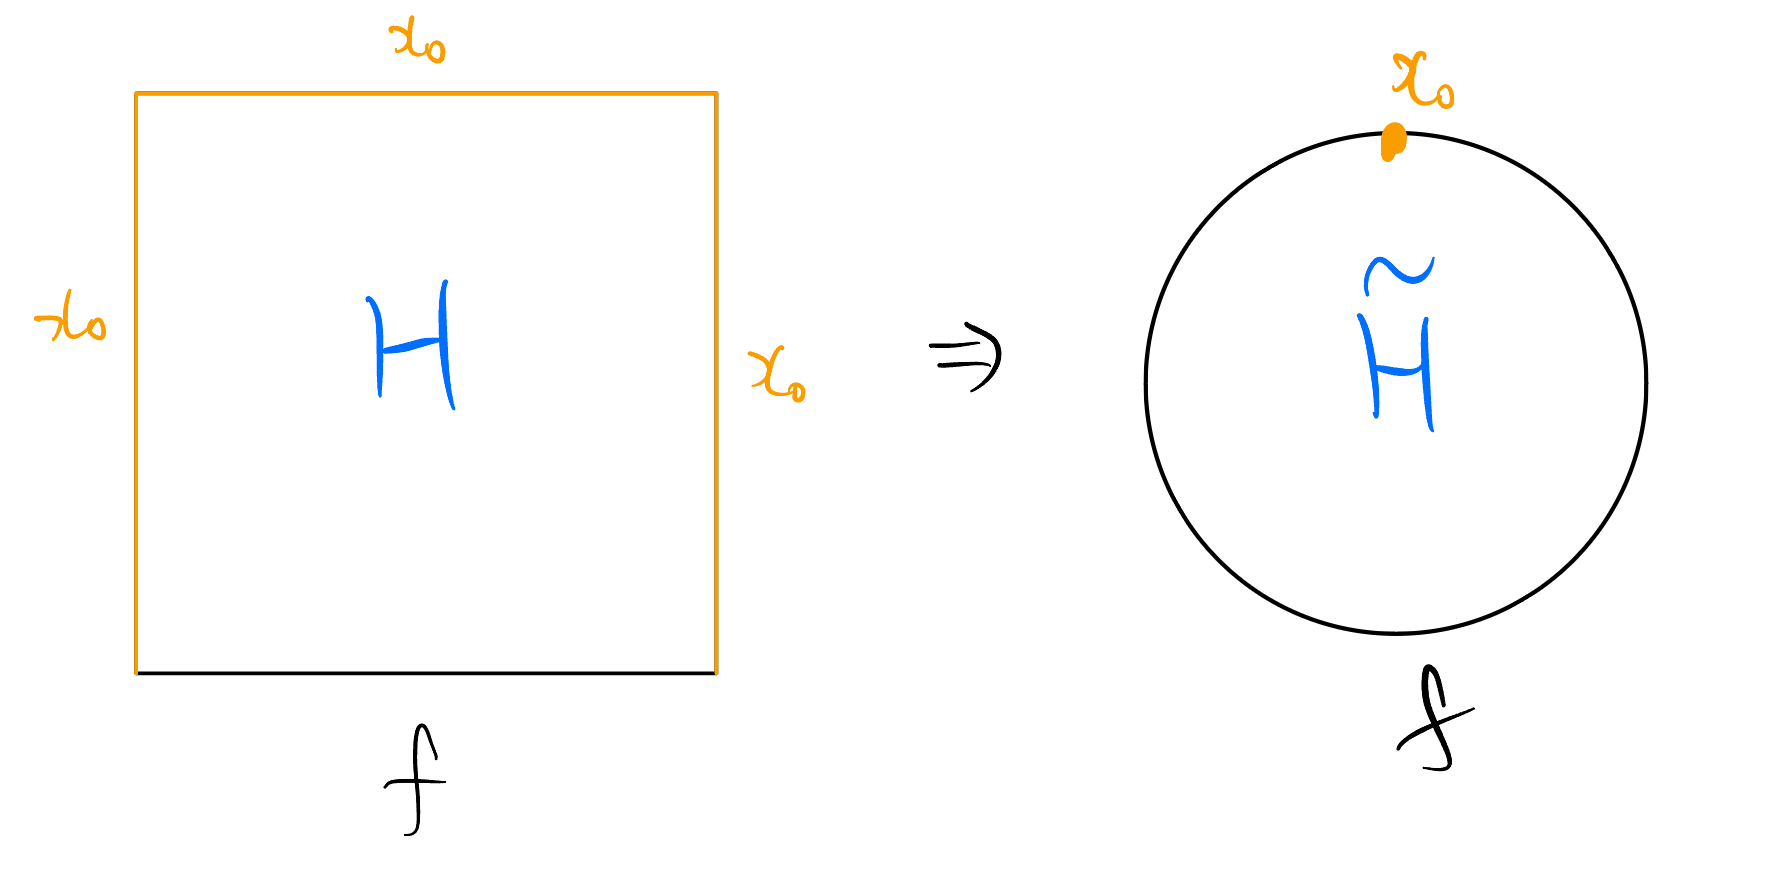
\includegraphics[width=0.8\textwidth]{./figures/extension.png}
	\caption{Nullhomotopic map extension.}
\end{figure}
 $ (\impliedby):$ Suppose $ X$ is path-connected, and every  $ f:S^{1} \to X$ extends to $ F:D^2 \to X$. Since $ D^2$ is contractible, by Homework 1 Problem 2, $ F$ is null-homotopic, and restricting the domain(which preserves continuity of the homotopy) yields that  $ f$ is also null-homotopic. That is,  $ \pi_1(X)$ is trivial. It follows from path-connectedness that $ X$ is simply connected.
\end{problem}

\begin{problem}[5]
	Given $ [f] \in [S^{1}, X]$ with representative $ f$ and $ p \in S^{1}$, denote $ x_1 = f(p)$. Since $ X$ is path-connected, let  $ \gamma$ be a path between $ x_0$ and $ x_1$, then $g:= \gamma * f * \overline{ \gamma}$ represents a based homotopy class in $ \pi_1( X,x_0)$. By forgetting about the base point via $ \Psi$, $ \Psi([g])$ becomes an element of $ [S^{1},X]$. We can clearly homotope $ \Psi(g)$ and  $ f$ by retracting  $ \gamma$ to the constant path at $ x_1$. Thus $ \Psi([g]) = [f]$ so $ \Psi$ is surjective.

~\begin{figure}[H]
	\centering
	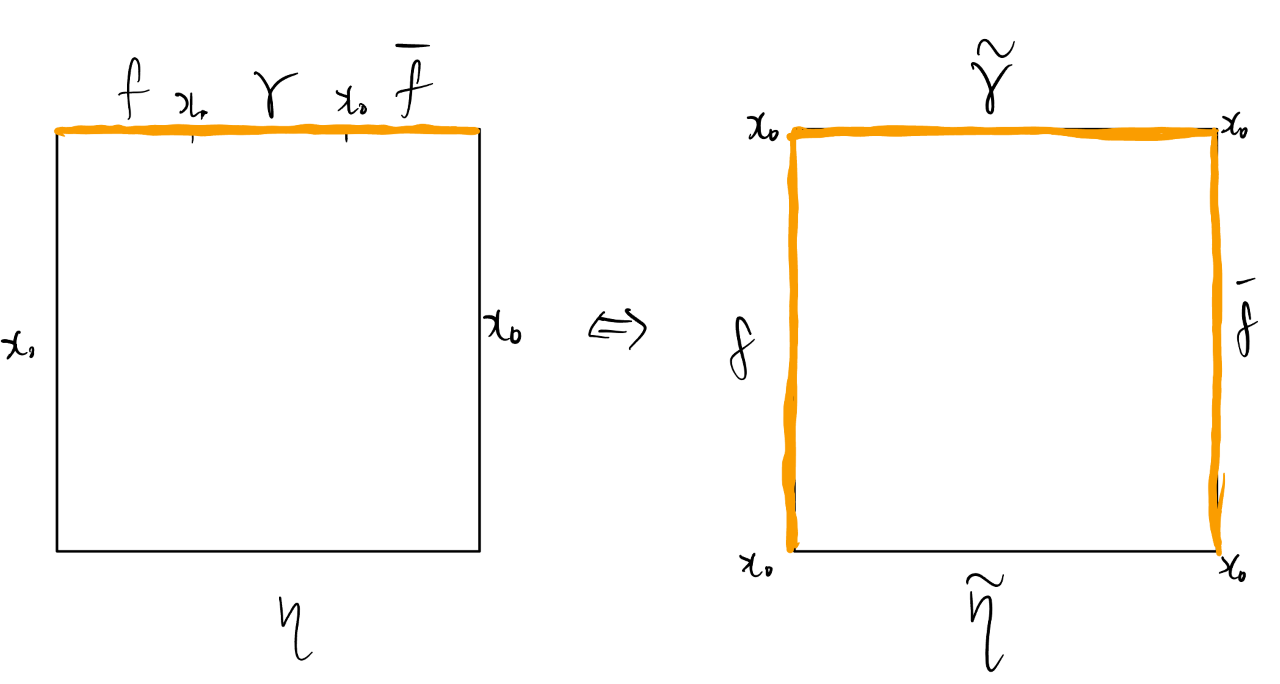
\includegraphics[width=0.7\textwidth]{./figures/unbased.png}
	\caption{Based vs unbased homotopy.}
\end{figure}
$ (\implies):$ Suppose $ \widetilde{ \gamma}:=\Psi([ \gamma]) = \Psi([\eta]):= \widetilde{ \eta}$. Then there exists a homotopy $ \widetilde{ H}: S^{1} \times I \to X$ between $ \widetilde{ \eta}$ and $ \widetilde{ \gamma}$, it is a square with vertical edges identified (or a cylinder), as depicted on the right in Figure 2. Notice that $f:= H|_{ \{p\} \times I}$ is a loop containing $ x_0$, so we can view it as a representative in $ \pi_1( X,x_0)$. Moreover, $ [f] = [\overline{f}]$ in $ [S^{1},X]$ since we can reparameterize the loop without respecting base point. Notice the two squares are clearly homotopic equivalent. We can stretch or shrink the orange boundary to the desired place in a continuous fashion (it would be easier to see via a homeomorphism to the disk), obtaining a homotopy rel boundary in based category as desired.

	$ (\impliedby):$ Suppose $ [ \gamma]$ and $ [ \eta]$ are conjugates in $ \pi_1( X,x_0) $, \emph{i.e.} $ [ \eta] = [f * \gamma * \overline{f}]$ for some $ [f] \in \pi_1( X,x_0) $. Then we get a homotopy as depicted on the left and collapse entire vertical edges to a single point $ x_0$ (the edges are contractible so it is indeed a homotopic equivalence) and map the orange part homeomorphically to get a homotopy in the unbased category on the right.
\end{problem}

\begin{problem}[6]
	Denote the Mobius strip by $ M$. As described by Figure 2, we can deformation retract $ M$ to its central circle $ C$ via the homotopy $ D: M \times I \to M, ([t,s],a) \mapsto [t, s(1-a)+ a/2]$. Let $ [f]$ be the generator of  $ \pi_1( C)$ which is also the generator of $ \pi_1( M)$ by inclusion. Since $ \partial M$ is also a circle, $ \pi_1( \partial M) \cong \zz$, generated by going around $ \partial M$ once, say $ [ g]$. Then we see that $g \simeq 2 f$ via $ D$.
~\begin{figure}[H]
	\centering
	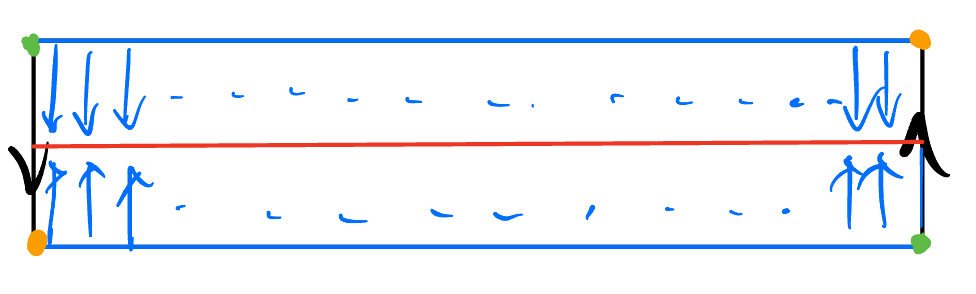
\includegraphics[width=0.8\textwidth]{./figures/mobius.png}
	\caption{We can view $ M$  as $ I^2$ with one pair of edges identified in opposing direction. Then it is clear that when we retract a loop (blue) around $ \partial M$ to the center circle $ C$, we get a loop (red) wrapping around  $ C$ twice via the homotopy in the figure.}
\end{figure}
	Suppose such retraction exists: $ r: M \to \partial M$. Let $ i: \partial M \to M$ be the inclusion map. Since $ r \circ i = \text{id}_{ \partial M}$ by the definition of retraction, by functoriality of $ \pi_1$, $ r_* \circ i_* = \text{id}_{ \pi_1( \partial M) }$. It follows that $ r_*: \zz \cong \pi_1( M) \to \pi_1( \partial M) \cong \zz$ is surjective. By the first isomorphism theorem, this forces $ \ker r_*$ to be trivial so $ r_*$ is injective as well, \emph{i.e.} it is an isomorphism that sends generator to generator, \emph{i.e.} $ [f] \mapsto [g]$. Since $ g \simeq 2f$, we see that $ r_* ([f]) = [2f] = 2 [f]$, contradicting that $ r_*$ is injective. 
\end{problem}
\begin{problem}[7]
	Given $ [\gamma], [\eta] \in \pi_1( G,e)$, it is straightforward to check that $ \gamma * \eta \simeq \gamma \cdot \eta$ by the following homotopy:
	\begin{align*}
		H(t,s) &= \begin{cases}
			\gamma \left( \frac{t}{s /2} \right) & 0 \leq t \leq \frac{s}{2} \\
			\gamma \cdot \eta \left( \frac{t- s /2}{ 1-s} \right) & \frac{s}{2} \leq t \leq 1- \frac{s}{2}\\
			\eta \left( \frac{t -1 + s /2}{ s /2} \right) & 1- \frac{s}{2} \leq t \leq 1\\
		\end{cases} 
	\end{align*}
In particular, the three clearly continuous piecewise functions agree on the basepoint so $ H$ is continuous by the pasting lemma.
~\begin{figure}[H]
	\centering
	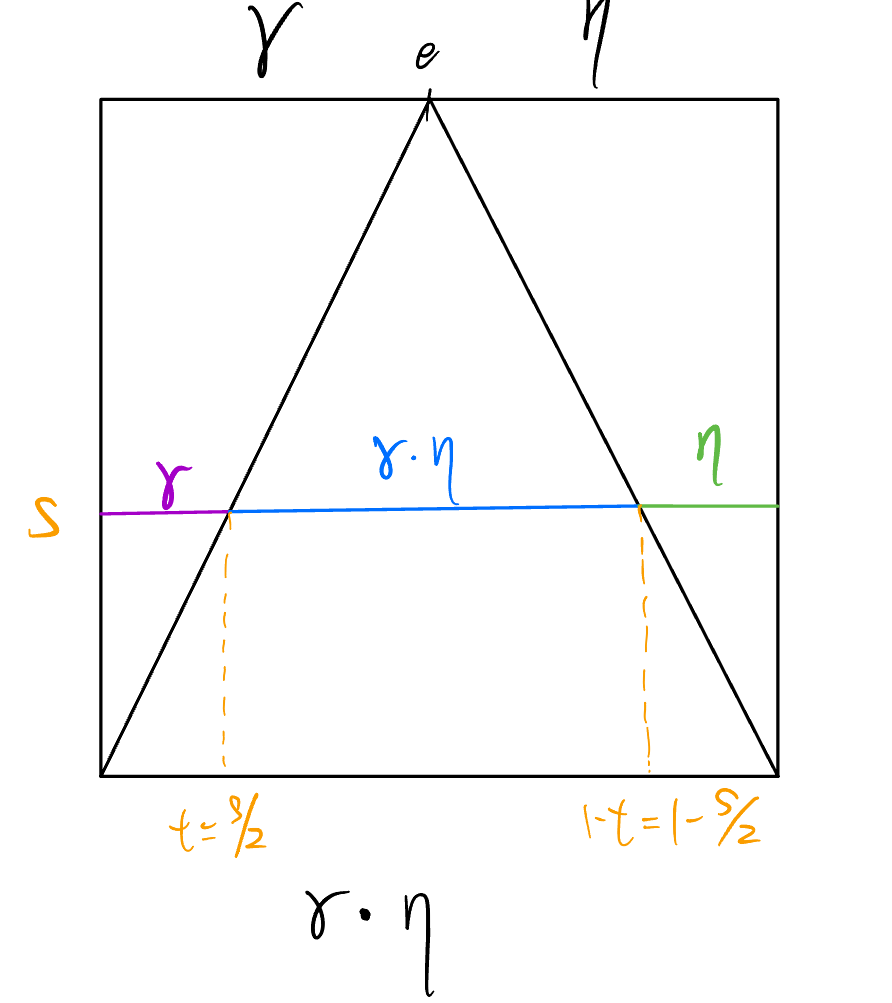
\includegraphics[width=0.4\textwidth]{./figures/abelian.png}
\end{figure}
\end{problem}
\begin{problem}[8]
Notice in problem 7 we could swap the order of $ \gamma$ and $ \eta$ and obtain a homotopy between $ \eta* \gamma$ and $ \gamma \cdot \eta$: 
	\begin{align*}
		H(t,s) &= \begin{cases}
			\eta \left( \frac{t}{s /2} \right) & 0 \leq t \leq \frac{s}{2} \\
			\gamma \cdot \eta \left( \frac{t- s /2}{ 1-s} \right) & \frac{s}{2} \leq t \leq 1- \frac{s}{2}\\
			\gamma \left( \frac{t -1 + s /2}{ s /2} \right) & 1- \frac{s}{2} \leq t \leq 1\\
		\end{cases} 
	\end{align*}

	Hence $\eta * \gamma \simeq \gamma \cdot \eta \simeq \gamma * \eta$. That is, $ [ \gamma] * [\eta] = [ \gamma \cdot \eta] = [\eta] * [ \gamma]$.

\end{problem}

\begin{problem}[15]
	Finite direct sum is isomorphic to the direct product, so $ \zz \oplus \zz \cong \zz^2$, which is the free abelian group (or free $ \zz$-module) on two generators. It suffices to show that $ G= \langle x,y| [x,y] \rangle$ satisfies the universal property of free abelian group on two generators. Given $ A$ and abelian group and any set map  $ \phi: \{x,y\} \to A, x \mapsto a, y \mapsto b$, we can construct an abelian group homomorphism $ \Phi: G \to A, x\mapsto a, y \mapsto b$. It suffices to check that the image satisfies the relations of $ G$:  $\Phi(x)\Phi(y)\Phi(x^{-1})\Phi(y^{-1}) = aba^{-1}b^{-1} = e_A= \Phi(e_G)$, which is valid because $ A$ is abelian. Since  $ G$ satisfies the universal property of free abelian group on two generators,  $ G \cong \zz^2$ so $ \zz \oplus \zz \cong \zz^2$ has the presentation $ G$.
\end{problem}
\end{document}
